\section{Data and unfolding methodology}
\label{sec:part-method}

% Bibliography mappings for keys introduced in this section:
% Andreopoulos:2009rq         arXiv:0905.2517
% GEANT4:2002zbu              doi:10.1016/S0168-9002(03)01368-8
% Nachman:2025staypositive    doi:10.1103/yx16-h7n9

\subsection{MINERvA data, simulation, and event selection}
\label{sec:minerva-data}
\label{sec:experiment}

MINERvA was a fine-grained scintillator detector in the NuMI beam at Fermilab,
immediately upstream of the MINOS near detector~\cite{MINERvA:2013zvz}. The central
scintillator tracker provides the hydrocarbon target and reconstructs the interaction
vertex and outgoing charged tracks. The tracker and electromagnetic calorimeter
measure energy deposited by the hadronic recoil. The downstream MINOS spectrometer
measures the charge and momentum of muons matched to MINERvA tracks. We use the
medium-energy neutrino-mode exposure, taken with forward horn current, for which the
mean neutrino energy is about \SI{6}{GeV}~\cite{MINERvA:2016iqn}. The flux is the
prediction used for the published cross section. It includes the PPFX hadron-production
reweighting of the NuMI simulation and the constraint from neutrino--electron
scattering~\cite{MINERvA:2016iqn,MINERvA:2021owq}.

\phantomsection
\label{sec:evloop}
The analyzed files span twelve run periods and contain $1.0574\times10^{21}$ protons
on target (POT). The published analysis quotes $1.061\times10^{21}$ POT. Our
selection yields $4\,119\,797$ reconstructed data events. We use GENIE
2.12.6~\cite{Andreopoulos:2009rq} to generate the reference sample. We apply
MINERvA Tune v1 as an event weight using the MINERvA Analysis Toolkit. Simulated
events pass through the Geant4-based MINERvA detector simulation~\cite{GEANT4:2002zbu}.
We apply the same reconstruction and selection to simulation and data. Simulated
event weights include the scaling to the data exposure. We pair each selected
simulated signal event with its generator record to transfer weights between
detector and truth levels. The denominator for the selection efficiency is the
full sample of $32\,849\,103$ generated signal events, including those that fail
reconstruction or selection.

\phantomsection
\label{sec:selection}
The signal follows the published inclusive charged-current (CC) $\nu_\mu$ definition
on hydrocarbon~\cite{MINERvA:2021owq}. The true vertex must lie within the central
tracker fiducial volume, $5980<z<\SI{8422}{mm}$ and within an apothem of
\SI{850}{mm}. This volume contains $3.2353\times10^{30}$ nucleons. The true
muon must satisfy
\begin{equation}
  \theta_\mu<20^\circ,\quad
  1.5<p_\parallel<\SI{60}{GeV/c},\quad
  p_T<\SI{4.5}{GeV/c} .
  \label{eq:muon-fiducial}
\end{equation}
The reconstructed selection requires a vertex in the same fiducial volume and a muon
at $\theta_\mu<20^\circ$ matched to a successfully fitted MINOS track. Antineutrino
candidates and events overlapping detector dead time
are rejected. These requirements apply at every unfolding dimension. The background
template includes selected neutral-current events, other-flavor or wrong-sign CC
interactions, interactions outside the fiducial volume, and CC $\nu_\mu$ events that
enter the reconstructed sample from outside the true muon phase space. On the 2D
reconstructed grid, the template accounts for \SI{2.91}{\percent} of the selected data yield,
ranging from \SI{2.72}{\percent} to \SI{3.23}{\percent} across run periods.

\phantomsection
\label{sec:controlplots}
Figure~\ref{fig:control} compares data and simulation at reconstruction level.
Appendix~\ref{app:higher-dimensional-projections} gives the correlations among the observables
(Fig.~\ref{fig:control-corner}).

\begin{figure}[H]
  \centering
  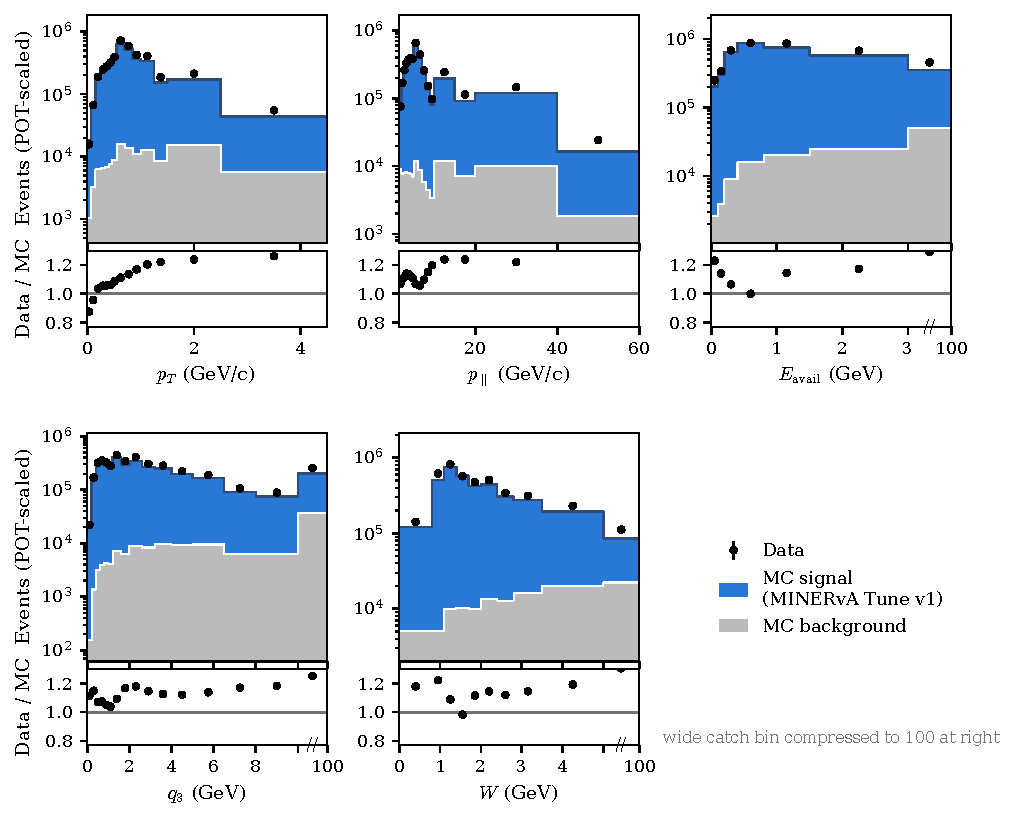
\includegraphics[width=\textwidth]{control_plots}
  \caption{Reconstructed $p_T$, $p_\parallel$, $E_{\mathrm{avail}}$, $q_3$, and $W$
  in data and in the sum of simulated signal and background at the data exposure.
  The data yield is about \SI{12}{\percent} higher overall. The data-to-simulation ratio in
  $p_T$ rises from 0.88 in the lowest bin to about 1.2 above \SI{1}{GeV/c}.}
  \label{fig:control}
\end{figure}

\subsection{Observable definitions}
\label{sec:observable-definitions}
\label{sec:eavailw-definitions}

At truth and reconstruction level, the muon observables are $p_T=p_\mu\sin\theta_\mu$
and $p_\parallel=p_\mu\allowbreak\cos\theta_\mu$, with $\theta_\mu$ measured from the beam
axis. The reconstructed values use the MINERvA--MINOS matched muon. In the remaining
definitions we use units with $c=1$.

\phantomsection
\label{sec:3d-method}
\label{sec:eavail-definition}
The true available energy is a sum over final-state protons, charged and neutral
pions, and photons,
% amsmath defers one display label. Its saved label command writes the legacy alias.
\begin{equation}
  \begin{aligned}[b]
    E_{\mathrm{avail}}^{\mathrm{true}}
    &= \sum_p (E_p-938.27\,\mathrm{MeV})\\
    &\quad + \sum_{\pi^\pm}(E_{\pi^\pm}-135\,\mathrm{MeV})
           + \sum_{\pi^0} E_{\pi^0} + \sum_\gamma E_\gamma .
  \end{aligned}
  \label{eq:available-energy-true}
  \csname ltx@label\endcsname{eq:eavail-implemented}
\end{equation}
The sum counts proton kinetic energy and the full energy of neutral pions and
photons. The charged-pion term uses a fixed \SI{135}{MeV} offset. Neutrons
and all other species outside the sum are omitted, so $E_{\mathrm{avail}}$ captures
only part of the hadronic energy transfer. The reconstructed quantity uses the
tracker and electromagnetic calorimeter (ECAL) deposits after removing energy
attributed to the muon,
\begin{equation}
  E_{\mathrm{avail}}^{\mathrm{reco}} =
  1.17 \sum_d \bigl(E_{\mathrm{dep}}^d-E_{\mu,\mathrm{dep}}^d\bigr),
  \label{eq:available-energy-reco}
  \csname ltx@label\endcsname{eq:eavail-reco-implemented}
\end{equation}
where $d$ runs over the tracker and ECAL. The reconstruction retains negative values
of this estimator.

The true magnitude of the three-momentum transfer is
$q_3^{\mathrm{true}}=\sqrt{Q^2+(E_\nu-E_\mu)^2}$, with $Q^2=-(k-k')^2$ evaluated
from the generator neutrino and muon four-momenta $k$ and $k'$.
\phantomsection\label{sec:eavailw-axis}%
For the true hadronic invariant-mass estimator we use
\begin{equation}
  W^{\mathrm{true}} = \bigl[
    M^2+2M(E_\nu-E_\mu)-4E_\nu E_\mu\sin^2(\theta_\mu/2)
  \bigr]^{1/2},
  \label{eq:hadronic-mass-true}
\end{equation}
where $M$ is the struck-nucleon mass and the last term uses the massless-muon
approximation for $Q^2$. Events with a negative radicand account for
$4.9\times10^{-5}$ of the simulated signal weight and are excluded from the
five-observable truth sample and its normalization.

At reconstruction level, $q_0^{\mathrm{reco}}$ is a separate calorimetric estimate of
the energy transfer. It does not use the factor 1.17 in
Eq.~\eqref{eq:available-energy-reco}. With reconstructed muon kinematics, the
definitions are
\begin{equation}
  \begin{aligned}[b]
    E_\nu^{\mathrm{reco}} &= E_\mu+q_0^{\mathrm{reco}},\\
    Q^2_{\mathrm{reco}} &=
      \max\{0,\,2E_\nu^{\mathrm{reco}}(E_\mu-p_\parallel)-m_\mu^2\},\\
    q_3^{\mathrm{reco}} &= \sqrt{Q^2_{\mathrm{reco}}+(q_0^{\mathrm{reco}})^2},\\
    W^{\mathrm{reco}} &=
      \sqrt{\max\{0,\,\bar M^2+2\bar M q_0^{\mathrm{reco}}-Q^2_{\mathrm{reco}}\}},
  \end{aligned}
  \label{eq:transfer-mass-reco}
  \csname ltx@label\endcsname{eq:shared-reco-inputs}
\end{equation}
where $m_\mu$ is the muon mass and $\bar M=(1.5M_n+M_p)/2.5$ is the effective
nucleon mass used in reconstruction. The inputs $(p_T,p_\parallel,q_3^{\mathrm{reco}})$
fix $W^{\mathrm{reco}}$, including its assignment to zero for \SI{1.5}{\percent} of simulated
events, so $W$ adds no independent detector input.

\subsection{OmniFold implementation and background subtraction}
\label{sec:omnifold-implementation}
\label{sec:method}
\label{sec:method-algo}

OmniFold estimates the truth distribution by iteratively reweighting simulated
events with classifier-based likelihood ratios~\cite{Andreassen:2019cjw,Andreassen:2021zzk}.
In the first step, a classifier distinguishes the background-corrected measured
sample from selected simulated signal carrying the current weights. For a classifier
probability $p$ for the measured class, the odds $p/(1-p)$ estimate the ratio of the
two weighted densities with the corresponding class normalization. The current
weight of each selected signal event is multiplied by this ratio and transferred to
its paired truth record. In the second step, a classifier compares the reweighted
truth sample with the original truth sample. Its likelihood ratio gives the new
truth weights relative to the original simulation. These weights are carried to the
matched detector-level records for the next iteration.

Truth signal events without a selected reconstructed partner enter the second step.
At each iteration, a regressor trained with uniform training weights on matched
events predicts their first-step weights from the truth observables. This procedure
incorporates the selection-efficiency correction into the reweighted truth sample.
It relies on the simulated acceptance and on transferring the weight inferred for
matched events to missed events at the same values of the truth inputs. Where the
simulated selection efficiency is very low, the estimate depends on the regressor's
extrapolation from matched events. The classifiers train and evaluate on the full
samples, without a held-out split, cross-fitting, or early stopping. We use five
iterations with gradient-boosted trees. The number of iterations and the learner
capacity regularize the weight estimate. The final truth weights can be integrated
on any of the reporting grids.

Background enters the measured class in the first step. Let $D(x)$ and $B(x)$ be the
selected data and exposure-scaled background densities in reconstructed coordinates
$x$, with integrals $D_b$ and $B_b$ in reconstructed bin $b$. The binned purity
method assigns the same weight to each data event in an occupied bin,
\begin{equation}
  w_{\mathrm{pur}}(b)=\frac{\max(0,D_b-B_b)}{D_b} .
  \label{eq:purity-weight}
\end{equation}
The classifier still uses the continuous event coordinates. Within a bin it sees
the data shape rescaled by a constant, $D(x)w_{\mathrm{pur}}(b)$.

Negative-weight subtraction keeps unit weights on the data and appends the simulated
background with the negative of its exposure-scaled event weights. In regions with
positive net density, the target first-step ratio is $[D(x)-B(x)]/S(x)$, where $S(x)$
is the current weighted density of selected simulated signal. In the binned limit,
in populated bins with $S_b>0$ and $D_b\geq B_b$, both treatments give the same
target mass $D_b-B_b$. An unbinned classifier can resolve shape differences within a
bin between $D(x)-B(x)$ and the purity-rescaled data.

The refined estimators convert the signed sample to nonnegative weights before the
first OmniFold classifier is trained. A separate classifier, trained with absolute
event weights, estimates the probability $g(x)$ that an event in the signed sample
has positive weight. The original weight $w$ is replaced by
$|w|\max\{0,2g(x)-1\}$~\cite{Nachman:2025staypositive}. The absolute-weight
sample has density $D+B$. In the population limit $g=D/(D+B)$, so multiplying this
density by the clipped factor gives the positive part of $D-B$. The learned factor
implements this prescription without a reconstructed subtraction grid. Appendix~\ref{app:negative-weight-background}
gives the binned limit and compares the two background treatments.

\subsection{Estimators and cross-section extraction}
\label{sec:estimators-and-extraction}
\label{sec:method-config}

The two-dimensional (2D) benchmark uses $(p_T,p_\parallel)$. The 3D, 4D, and 5D
unfoldings add $E_{\mathrm{avail}}$, $q_3$, and $W$ in sequence at both reconstruction
and truth level. Table~\ref{tab:estimators} identifies the estimator for each result
and for the diagnostic studies that use a different configuration.

\begin{table}[!t]
  \centering\small
  \caption{Estimators, reporting grids, and diagnostics. Background treatment
  refers to the first OmniFold step.}
  \label{tab:estimators}
  \label{tab:estimators-matrix}
  \label{tab:config-key}
  \begin{tabular}{@{}>{\raggedright\arraybackslash}p{0.25\textwidth}
                      >{\raggedright\arraybackslash}p{0.31\textwidth}
                      >{\raggedright\arraybackslash}p{0.38\textwidth}@{}}
    \toprule
    Result or diagnostic & Estimator and background treatment & Grid and covariance or test statistic \\
    \midrule
    2D muon cross section &
      \EstTwoD{} (refined negative weights) &
      Published muon grid (\lrval{q-ncells} bins) with covariance $Q_R$. \\
    \addlinespace
    3D and 4D central values &
      \EstMultiD{} (refined negative weights) &
      Central values on fine muon and hadronic grids. \\
    \addlinespace
    Exploratory five-axis result &
      \EstPurity{} (binned purity weights) &
      Fine five-axis grid with diagnostic covariance $C_Z$, also projected
      onto the $E_{\mathrm{avail}}$--$W$ plane. \\
    \addlinespace
    Sixteen-cell result (illustrative) &
      \EstMultiD{} (refined negative weights) &
      Merged reporting regions with covariance $C_{\mathrm{rep}}$. \\
    \addlinespace
    Joint generator tests &
      Variant of the \estMultiD{} (refined negative weights) &
      Separate coarse grid with \jtNcells{} supported cells
      (\jtNcellsGiBUU{} for GiBUU). Calibrated quadratic distances use
      a shrinkage-based metric. \\
    \midrule
    \multicolumn{3}{@{}l}{\emph{Diagnostic controls}} \\
    Injected-feature closures and classifier-family cross-check &
      \EstPurity{} (binned purity weights) & \\
    \addlinespace
    Background-subtraction bias and 5D coverage &
      \EstDetPurity{} (binned purity weights) & \\
    \addlinespace
    Background-subtraction bias and generator-sized available-energy change &
      \EstLowCap{} (refined negative weights) & \\
    \addlinespace
    2D unfolding cross-check &
      \EstExact{} (binned purity weights) &
      Published muon grid. \\
    \bottomrule
  \end{tabular}
\end{table}

\phantomsection
\label{sec:method-xsec}
For a truth bin $i$, let $U_i$ be the unfolded yield. We obtain the flux-averaged,
bin-integrated cross section per nucleon as
\begin{equation}
  \sigma_i = \frac{U_i}{\Phi_i N_{\mathrm{nuc}}N_{\mathrm{POT}}} .
  \label{eq:flux-averaged-cross-section}
\end{equation}
Here $N_{\mathrm{nuc}}$ is the fiducial nucleon count and $N_{\mathrm{POT}}$ is the
analyzed exposure.
The cross-section density is $\sigma_i$ divided by the product of its bin widths. Every extraction uses the integrated flux tabulated by $p_T$ bin
and broadcast over the other axes. Integrated over $0<E_\nu<\SI{100}{GeV}$
after the constraint, it is
\SI{6.243e-8}{cm^{-2}} per POT.
% Check stage (2026-11-21): nd-unfolding/xsec_nd.py (flux per p_T bin, broadcast over every other axis) and
% docs/orchestration/state/s5p/gen5d/README-gen5d-fluxfix.md:74 (Phi_t = 6.243343e-4 m^-2/POT = hFluxCV, every p_T bin equal). The sum $U_i$ includes
reweighted signal events missed by the selection,
so the truth-sample completeness factor in the extraction is unity in every bin.

\phantomsection
\label{sec:method-binning}
The 2D result follows the published $14\times16$ muon grid and its mapping of 205
reported bins~\cite{MINERvA:2021owq}. The remaining 19 cells lie in the high-$p_T$,
low-$p_\parallel$ corner, with $p_T^{\mathrm{hi}}/p_\parallel^{\mathrm{lo}}>\tan20^\circ$. The higher-dimensional fine
grids add seven $E_{\mathrm{avail}}$ bins, seven $q_3$ bins, and six $W$ bins, each
with a wide final bin extending to 100 in its respective axis units. Appendix~\ref{app:reproducibility}
gives the bin edges. A marginal cross section sums the bin integrals over the eliminated
axes and divides by the retained bin widths when reported as a density. The wide
bins contribute their full integrals to projections and totals.

The 3D and 4D results are reported as central values only. The covariance of the
\resFiveAxis{} serves as a scale for diagnostics. The \resSixteen{}
uses coarser regions of the joint phase space, defined in Sec.~\ref{sec:five-dimensional-reporting}. It is
expressed as integrated cross sections in $\mathrm{cm}^2$ per nucleon and is
reported with its covariance for illustration. The calibrated generator tests in
Sec.~\ref{sec:sixteen-cell-generator-comparison} apply a variant of the multidimensional estimator on a separate joint grid.
The records document~\cite{NoteRecords2026} gives further qualifications of the
selection, the training settings, and the estimator configurations.

% PASS2:
% Numbers: the supplied source prints the quantitative values as literals, including
% the numerical arguments of \SI. The published POT here (1.061 x 10^21) is the same
% literal value that sec_experiment.tex writes as 10.61 x 10^20. The seven q_3 bins
% are confirmed in the original note's Appendix D.1.2, whose TeX is not in inputs2.
% References: all retained references have targets in this file or new-labels.md.
% The former selection-features, observable-definitions, and 3D-configuration tables
% (tab:selection-features, tab:observables-impl, tab:3d-configs) and the separate driver
% subsection (sec:method-driver) have no retained equivalent floats or heading here.
% The corner plot is assigned to Appendix C.2. The migration plot (fig:migration) is
% absent from the rewritten section and has no destination in the supplied label map.
% Figure asset: control_plots.pdf is listed in figures.txt, but not staged in inputs2.
